\documentclass[../piano-di-progetto.tex]{subfiles}

\begin{document}

\section{Analisi dei rischi}
Durante lo sviluppo di un progetto complesso, è possibile incorrere in problemi che potrebbero essere evitati tramite un processo preliminare di analisi dei rischi. Con l'obiettivo di prevenire ed evitare queste evenienze, è stata effettuata un'attenta analisi dei principali fattori di rischio svolgendo i seguenti passi:

\begin{itemize}
    \item \textbf{Identificazione dei rischi}: individuazione dei possibili fattori di rischio che potrebbero rallentare o bloccare il normale svolgersi del progetto;
    \item \textbf{Analisi dei rischi}: valutazione delle probabilità di occorrenza del rischio, valutazione delle ripercussioni sul progetto e, infine, assegnazione di un indice di grado del rischio;
    \item \textbf{Pianificazione di controllo}: definizione della metodologia per evitare di incorrere nei rischi individuati e come procedere nell'eventualità in cui non sia possibile evitarne alcuni;
    \item \textbf{Monitoraggio dei rischi}: monitoraggio continuo al fine di rilevare quanto prima l'incombere di un rischio con l'obiettivo di poterlo evitare oppure limitare le ripercussioni sullo svolgersi del progetto.
\end{itemize}

\subsection{Valutazione}
Viene utilizzato il sistema a matrice di valutazione dei rischi. Ad ogni rischio viene associato un indice di gravità, ottenuto considerando la probabilità che tale rischio possa accadere e l'impatto che esso avrà sullo svolgersi del progetto. Questo indice può assumere i seguenti valori:
\begin{itemize}
    \item Basso;
    \item Medio;
    \item Alto;
    \item Critico.
\end{itemize}
\begin{figure}[H]
	\centering
	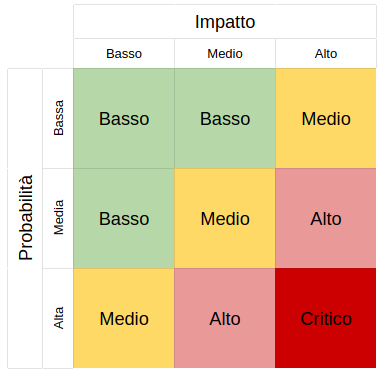
\includegraphics[width=10cm]{img/matrice-rischio.png}
	\caption{Matrice dell'indice di gravità del rischio}
	\label{fig:matrice-rischio}
  \end{figure}

\subsection{Classificazione}
Ad ogni rischio viene assegnato un codice univoco affinché possa essere identificato e facilmente riconoscibile. La struttura del codice identificativo è la seguente: \\
\texttt{RK-[Categoria]-[ID]-[Indice di gravità]} \\
I tre campi assumono i seguenti valori:
\begin{itemize}
    \item \textbf{Categoria}:
        \begin{itemize}
            \item \textbf{O}: Organizzativo;
            \item \textbf{P}: Personale;
            \item \textbf{T}: Tecnologico.
        \end{itemize}
    \item \textbf{ID}: rappresenta un numero intero incrementale all'interno della categoria;
    \item \textbf{Indice di gravità}: valore ottenuto dalla matrice in figura \ref{fig:matrice-rischio} con la seguente associazione:
        \begin{itemize}
            \item \textbf{1}: Basso;
            \item \textbf{2}: Medio;
            \item \textbf{3}: Alto;
            \item \textbf{4}: Critico.
        \end{itemize}
\end{itemize}

\subsection{Possibili rischi}
    \begin{longtable}[H]{ccc}
        \caption{Tabella dei rischi} \\
        \rowcolor{lightgray} 
        \textbf{Codice} & \textbf{Descrizione} & \textbf{Identificazione} \\

        \endfirsthead
        \multicolumn{3}{c}%
        {\tablename\ \thetable\ -- \textit{Continuazione della pagina precedente}} \\
        \rowcolor{lightgray}

        \textbf{Codice} & \textbf{Descrizione} & \textbf{Identificazione} \\

        \endhead
         \multicolumn{3}{r}{\textit{Continua alla prossima pagina}} \\
        \endfoot

        \endlastfoot
        \begin{tabular}[c]{@{}l@{}}RK-P1-3\\Inesperienza\\tecnologica\end{tabular} & \begin{tabular}[c]{@{}l@{}}Il Responsabile parlerà\\periodicamente con ogni\\membro del gruppo per capire\\le conoscenze del singolo\\individuo\end{tabular} & \begin{tabular}[c]{@{}l@{}}Ogni membro avviserà il\\Responsabile in caso di \\difficoltà\end{tabular}  \\
\textbf{Piano di contingenza}                                              & \multicolumn{2}{l}{\begin{tabular}[c]{@{}l@{}} Ogni membro si impegna a sanare i propri dubbi per \\poter lavorare in modo autonomo\end{tabular}}                                                                                                                     \\
\hline
        %%%%
 \begin{tabular}[c]{@{}l@{}} RK-P2-3\\ \\ Inesperienza \\ gestionale \end{tabular}                    & \begin{tabular}[c]{@{}l@{}}Nessun membro del gruppo si è mai trovato nelle \\ condizioni di lavorare ad un progetto di dimensioni \\ così elevate \end{tabular}                                               & \begin{tabular}[c]{@{}l@{}}Il Responsabile avrà il compito\\ di assicurarsi che ogni membro \\ del gruppo abbia compreso \\ pienamente il ruolo e i compiti a \\ lui assegnati \end{tabular}                                                                                                                                                                                                                                                                                                                                                                                                                                                                                             \\
\textbf{Piano di contingenza}                                                                        & \multicolumn{2}{l}{\begin{tabular}[c]{@{}l@{}}Ogni componente si impegna a studiare in modo autonomo i compiti e doveri associati \\ ad ogni ruolo e informare il Responsabile in caso di perplessità \end{tabular}}                                                                                                                                                                                                                                                                                                                                                                                                                                                                                                                                                                                                                                                                                     \\ 
\hline
\begin{tabular}[c]{@{}l@{}} RK-P3-3\\ \\ Impegni \\ accademici \end{tabular}                         & \begin{tabular}[c]{@{}l@{}}Alcuni membri del gruppo potrebbero non essere \\ sempre disponibili per continuare lo sviluppo \\ del progetto a causa di impegni accademici \end{tabular}                        & \begin{tabular}[c]{@{}l@{}}Il Responsabile verificherà \\ periodicamente lo stato degli \\ impegni accademici dei singoli \\ componenti \end{tabular}                                                                                                                                                                                                                                                                                                                                                                                                                                                                                                                                    \\
\textbf{Piano di contingenza}                                                                        & \multicolumn{2}{l}{\begin{tabular}[c]{@{}l@{}}Sarà compito dei singoli individui programmare gli impegni accademici in modo tale\\ che non interferiscano con lo svolgersi del progetto. Inoltre, il Responsabile a \\ conoscenza degli impegni accademici dei singoli, assegnerà compiti compatibili \\ con essi \end{tabular}}                                                                                                                                                                                                                                                                                                                                                                                                                                                                                                                                                                         \\ 
\hline
\begin{tabular}[c]{@{}l@{}} RK-P4-2\\ \\ Impegni \\ personali \end{tabular}                          & \begin{tabular}[c]{@{}l@{}}Alcuni membri del gruppo potrebbero essere \\ indisponibili a causa di impegni personali \end{tabular}                                                                             & \begin{tabular}[c]{@{}l@{}}I membri del gruppo dovranno \\ segnalare al Responsabile \\ eventuali indisponibilità \end{tabular}                                                                                                                                                                                                                                                                                                                                                                                                                                                                                                                                                          \\
\textbf{Piano di contingenza}                                                                        & \multicolumn{2}{l}{\begin{tabular}[c]{@{}l@{}}In caso di ritardi, sarà compito del Responsabile valutare una riassegnazione dei \\ compiti in modo da poter rispettare i tempi prestabiliti \end{tabular}}                                                                                                                                                                                                                                                                                                                                                                                                                                                                                                                                                                                                                                                                                               \\ 
\hline
\begin{tabular}[c]{@{}l@{}} RK-P5-2\\ \\ Abbandono \\ del gruppo \end{tabular}                       & \begin{tabular}[c]{@{}l@{}}Per motivi personali, un membro del gruppo \\ potrebbe decidere di abbandonare lo sviluppo \end{tabular}                                                                           & \begin{tabular}[c]{@{}l@{}}Il componente che intende \\ lasciare lo sviluppo deve \\ informare il prima possibile il\\ resto del gruppo \end{tabular}                                                                                                                                                                                                                                                                                                                                                                                                                                                                                                                                    \\
\textbf{Piano di contingenza}                                                                        & \multicolumn{2}{l}{\begin{tabular}[c]{@{}l@{}}Si valuterà se l'abbandono del gruppo da parte del componente potrà diventare \\ solo un temporaneo congedo \end{tabular}}                                                                                                                                                                                                                                                                                                                                                                                                                                                                                                                                                                                                                                                                                                                                 \\ 
\hline
\begin{tabular}[c]{@{}l@{}} RK-O1-3\\ \\ Calcolo dei \\ costi e \\ tempistiche \end{tabular}         & \begin{tabular}[c]{@{}l@{}}A causa delle dimensioni molto elevate del progetto \\ e dalla inesperienza dei membri del gruppo, le \\ stime dei tempi e dei costi potrebbero risultare incoerenti \end{tabular} & \begin{tabular}[c]{@{}l@{}}Ogni membro ha il compito di \\ informare il Responsabile nel \\ caso in cui il proprio compito \\ stia superando le ore previste \end{tabular}                                                                                                                                                                                                                                                                                                                                                                                                                                                                                                               \\
\textbf{Piano di contingenza}                                                                        & \multicolumn{2}{l}{\begin{tabular}[c]{@{}l@{}}Se le ore effettive richieste da un certo compito stanno per superare le ore \\ preventivate, verrà considerata una ripartizione di quest'ultimo \end{tabular}}                                                                                                                                                                                                                                                                                                                                                                                                                                                                                                                                                                                                                                                                                            \\ 
\hline
\begin{tabular}[c]{@{}l@{}} RK-O2-2\\ \\ Conflitti interni \end{tabular}                             & \begin{tabular}[c]{@{}l@{}}Potrebbero verificarsi situazioni di tensione \\ tra due o più membri del gruppo \end{tabular}                                                                                     & \begin{tabular}[c]{@{}l@{}}Appena questa situazione si \\ verifica, è compito dei membri\\ coinvolti mettere al corrente il\\ resto del gruppo \end{tabular}                                                                                                                                                                                                                                                                                                                                                                                                                                                                                                                             \\
\textbf{Piano di contingenza}                                                                        & \multicolumn{2}{l}{\begin{tabular}[c]{@{}l@{}}Il Responsabile, o un componente non coinvolto, assumerà l'incarico di \\ mediatore per risolvere la situazione \end{tabular}}                                                                                                                                                                                                                                                                                                                                                                                                                                                                                                                                                                                                                                                                                                                             \\ 
\hline
\begin{tabular}[c]{@{}l@{}} RK-O4-2\\ \\ Comunicazione \\ con il \\ proponente \end{tabular}         & \begin{tabular}[c]{@{}l@{}}Il proponente potrebbe non essere disponibile a causa \\ di impegni lavorativi \end{tabular}                                                                                       & \begin{tabular}[c]{@{}l@{}}Sin dal primo colloquio si \\ cercherà di capire le \\ disponibilità del proponente \end{tabular}                                                                                                                                                                                                                                                                                                                                                                                                                                                                                                                                                             \\
\textbf{Piano di contingenza}                                                                        & \multicolumn{2}{l}{\begin{tabular}[c]{@{}l@{}}Il gruppo cercherà di chiarire quanti più dubbi possibili durante ogni colloquio \\ preparando in anticipo una lista di domande \end{tabular}}                                                                                                                                                                                                                                                                                                                                                                                                                                                                                                                                                                                                                                                                                                             \\ 
\hline
\multicolumn{1}{c}{\begin{tabular}[c]{@{}c@{}} RK-O5-2\\\\Impossibilità di \\incontro \end{tabular}} & \begin{tabular}[c]{@{}l@{}}Per ragioni logistiche e personali, potrebbe essere\\difficile incontrarsi fisicamente con tutto il gruppo \end{tabular}                                                           & \begin{tabular}[c]{@{}l@{}}Gli incontri verranno organizzati\\in anticipo cercando data e \\luogo adatti \end{tabular}                                                                                                                                                                                                                                                                                                                                                                                                                                                                                                                                                                   \\
\textbf{Piano di contingenza}                                                                        & \multicolumn{2}{l}{\begin{tabular}[c]{@{}l@{}}Nel caso in cui non si riesca ad arrivare a un compromesso, verrà organizzato un incontro \\ telematico \end{tabular}}                                                                                                                                                                                                                                                                                                                                                                                                                                                                                                                                                                                                                                                                                                                                     \\ 
\hline
\begin{tabular}[c]{@{}l@{}} RK-T1-2\\ \\ Problemi software \\ e hardware \end{tabular}               & \begin{tabular}[c]{@{}l@{}}Qualcuno potrebbe riscontrare problemi software \\ o hardware all'interno del computer, non potendo \\ proseguire nell'immediato con lo sviluppo del progetto \end{tabular}        & \begin{tabular}[c]{@{}l@{}}Ogni componente dovrà \\ segnalare tempestivamente \\ il problema riscontrato \\ tramite un dispositivo non \\ affetto da guasti \end{tabular}                                                                                                                                                                                                                                                                                                                                                                                                                                                                                                                \\
\textbf{Piano di contingenza}                                                                        & \multicolumn{2}{l}{\begin{tabular}[c]{@{}l@{}}Nel caso la riparazione non potesse essere portata a termine in tempi molto brevi, il singolo \\ dovrà utilizzare un computer sostitutivo per continuare lo sviluppo. Nell'evenienza in cui il \\ componente non avesse a disposizione nessun dispositivo allora il Responsabile dovrà \\ procedere alla riassegnazione dei compiti \end{tabular}}                                                                                                                                                                                                                                                                                                                                                                                                                                                                                                         \\ 
\hline
\begin{tabular}[c]{@{}l@{}} RK-T2-4\\ \\ Guasti servizi\\ cloud \end{tabular}                        & \begin{tabular}[c]{@{}l@{}}Il gruppo ha deciso di utilizzare alcuni\\ servizi online forniti da terzi per la gestione\\ di alcuni aspetti del progetto \end{tabular}                                          & \begin{tabular}[c]{@{}l@{}}Appena un componente noterà\\ malfunzionamenti nei servizi,\\ dovrà avvisare l'intero gruppo \end{tabular}                                                                                                                                                                                                                                                                                                                                                                                                                                                                                                                                                    \\
\textbf{Piano di contingenza}                                                                        & \multicolumn{2}{l}{\begin{tabular}[c]{@{}l@{}}Ogni componenti avrà una copia dell'intero prodotto, se il guasto non dovesse essere risolto \\ dal provider in pochi giorni, si valuterà la migrazione ad un altro fornitore \end{tabular}}                                                                                                                                                                                                                                                                                                                                                                                                                                                                                                                                                                                                                                                               \\
\begin{tabular}[c]{@{}l@{}}RK-T3-4\\ Guasti di linea \end{tabular}                                   & \begin{tabular}[c]{@{}l@{}}Potrebbero verificarsi guasti e \\malfunzionamenti imprevisti nel funzionamento\\della linea internet dei componenti del gruppo \end{tabular}                                      & \begin{tabular}[c]{@{}l@{}}Appena un componente noterà\\ malfunzionamenti nella linea,\\ dovrà avvisare l'intero gruppo\\tramite SMS o chiamata\\ \end{tabular}                                                                                                                                                                                                                                                                                                                                                                                                                                                                                                                          \\
\textbf{Piano di contingenza}                                                                        & \multicolumn{2}{l}{\begin{tabular}[c]{@{}l@{}}Ogni componente che rileva malfunzionamenti alla propria linea internet \\dovrà cercare di connettersi a linee alternative come la rete 4G del telefono\\tramite funzione \glossario{hotspot}. Nel caso il componente non potesse tornare online\\nel breve tempo, il lavoro verrà riorganizzato in attesa che il malfunzionamento\\venga risolto. Nel caso in cui il membro abbia del lavoro in locale che non può\\pubblicare sugli appositi sistemi, si valuterà se la pubblicazione può essere \\ritardata considerando però che non c'è garanzia che la rete torni a funzionare.\\Se la pubblicazione non può essere ulteriormente rimandata, il componente \\dovrà contattare telefonicamente il responsabile per una descrizione del lavoro\\quanto più accurata possibile e quest'ultimo dovrà completare il lavoro o \\assegnarlo ad un terzo \end{tabular}} 
   
    
    \end{longtable}
\end{document}
